%* 
%* ------------------------------------------------------------------
%* Model Railroad System by Deepwoods Software
%* ------------------------------------------------------------------
%* MainGUI.tex - Main GUI
%* Created by Robert Heller on Fri Mar  8 22:43:29 2002
%* ------------------------------------------------------------------
%* Modification History: $Log$
%* Modification History: Revision 1.1  2002/11/09 21:21:07  heller
%* Modification History: Time Table User Manual
%* Modification History:
%* ------------------------------------------------------------------
%* Contents:
%* ------------------------------------------------------------------
%*  
%*     Model RR System, Version 2
%*     Copyright (C) 1994-2002  Robert Heller D/B/A Deepwoods Software
%* 			51 Locke Hill Road
%* 			Wendell, MA 01379-9728
%* 
%*     This program is free software; you can redistribute it and/or modify
%*     it under the terms of the GNU General Public License as published by
%*     the Free Software Foundation; either version 2 of the License, or
%*     (at your option) any later version.
%* 
%*     This program is distributed in the hope that it will be useful,
%*     but WITHOUT ANY WARRANTY; without even the implied warranty of
%*     MERCHANTABILITY or FITNESS FOR A PARTICULAR PURPOSE.  See the
%*     GNU General Public License for more details.
%* 
%*     You should have received a copy of the GNU General Public License
%*     along with this program; if not, write to the Free Software
%*     Foundation, Inc., 675 Mass Ave, Cambridge, MA 02139, USA.
%* 
%*  
%* 

\chapter{Main GUI}
\label{chapt:MainGUI}

Once you have loaded up your layout information, the main GUI window is
displayed, as shown in Figure~\ref{fig:mrrTTMain}.  The central portion
of the window contains your operating chart, with time along the top
from left to right and the stations along the left edge from top to
bottom.  Above the operating chart are the cabs and below the chart are
the storage tracks.  Below the chart area is a row of buttons and above
the chart is a menu bar.\footnote{Except under MacOS, where the menu bar
is wired to the top of the desktop screen.}

\begin{figure}
\begin{centering}
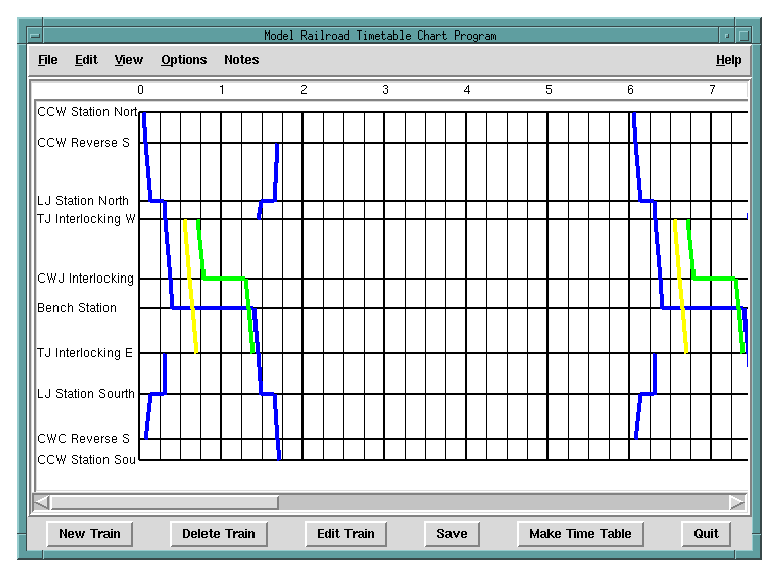
\epsfig{file=TimeTable/mrrTTMain.ps}\\
\caption{Main GUI window.}
\label{fig:mrrTTMain}
\end{centering}
\end{figure}

\section{Action Buttons}

\subsection{New Train button}

The {\tt New Train} button creates a new train.  See
Chapter~\ref{chapt:AddingTrains} for complete details on how to add a
new train.

\subsection{Delete Train Button}

The {\tt Delete Train} button is not implemented yet.

\subsection{Edit Train Button}

The {\tt Edit Train} button is not implemented yet.

\subsection{Save Button}

The {\tt Save} button saves the current file.  This is the same as the
{\tt Save} item on the {\tt File} menu.

\subsection{Make Time Table button}

The {\tt Make Time Table} button creates a hard copy time table.  See
Chapter~\ref{chapt:PrintingATimetable} for details.

\subsection{Quit button}

The {\tt Quit} button quits the application.  Same as the {\tt Close}
and {\tt Exit} items under the {\tt File} menu.


\section{Menu Bar}

\subsection{File Menu}

The {\tt File} menu follows the Motif Standard.

\subsubsection{New item}

This item clears out the current chart and creates a new one from scratch.

\subsubsection{Open\ldots\ item}

This item clears out the current chart and loads a chart saved on disk.

\subsubsection{Save item}

This item saves the current chart to the last file used to load or save
a chart.  If there is no current file, this item behaves like the {\tt
Save As\ldots} item.

\subsubsection{Save As\ldots\ item}

This item saves the current chart to a newly selected file name.

\subsubsection{Print\ldots\ item}

This item creates a hard copy time table.  See
Chapter~\ref{chapt:PrintingATimetable} for details.

\subsubsection{Close item}

This item is the same as the {\tt Exit} item and {\tt Quit} buttons.

\subsubsection{Exit item}

This item is the same as the {\tt Close} item and {\tt Quit} buttons.

\subsection{View Menu}

\subsubsection{Single Train item}

The {\tt Single Train} menu button displays the ``View Train'' pop-up
box, as shown in Figure~\ref{fig:viewSingleTrainPopup}.

\begin{figure}
\begin{centering}
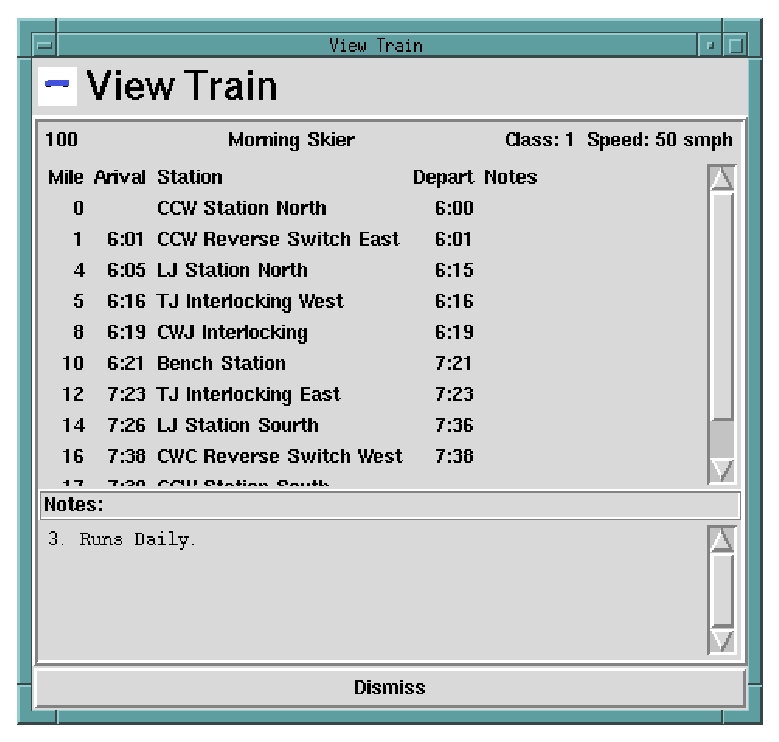
\epsfig{file=TimeTable/viewSingleTrainPopup.ps}\\
\caption{View Train Pop-up box.}
\label{fig:viewSingleTrainPopup}
\end{centering}
\end{figure}   

\subsubsection{All Trains item}

The {\tt All Trains} menu button displays the ``View All Trains'' pop-up
box, as shown in Figure~\ref{fig:viewAllTrainsPopup}. 

\begin{figure}
\begin{centering}
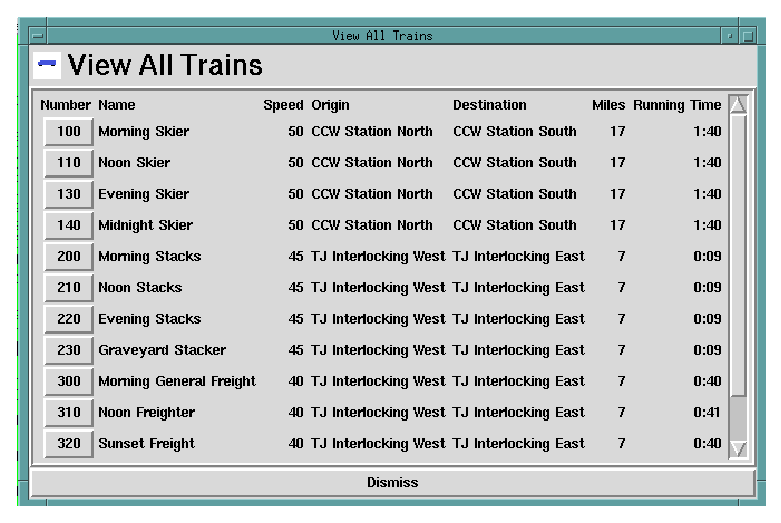
\epsfig{file=TimeTable/viewAllTrainsPopup.ps}\\
\caption{View All Trains Pop-up box.}
\label{fig:viewAllTrainsPopup}
\end{centering}
\end{figure}   

\subsubsection{Stations item}

The {\tt Stations} menu button displays the ``View Stations'' pop-up box,
as shown in Figure~\ref{fig:viewStations}.

\begin{figure}
\begin{centering}
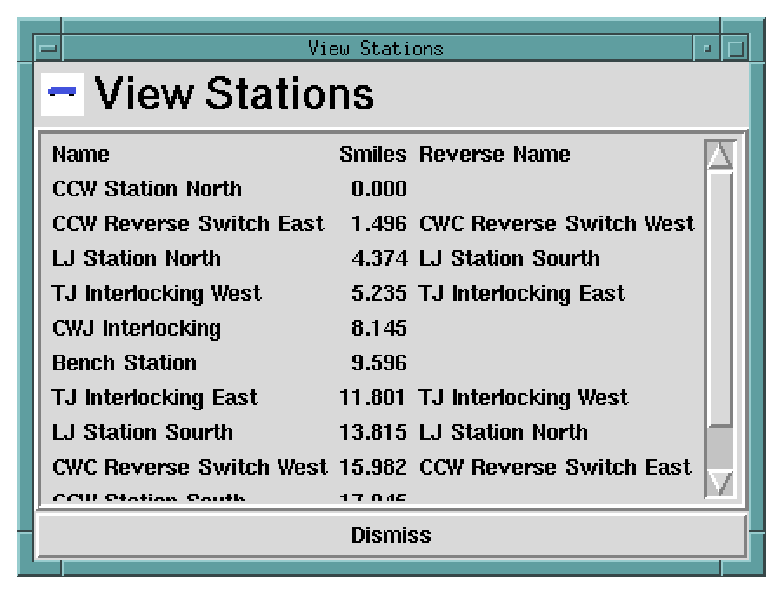
\epsfig{file=TimeTable/viewStations.ps}\\
\caption{View Stations Pop-up box.}
\label{fig:viewStations}
\end{centering}
\end{figure}   


\subsubsection{Cabs item}

The {\tt Cabs} menu button displays the ``View Cabs'' pop-up box.

\subsubsection{Storage Tracks item}

The {\tt Storage Tracks } menu button displays the ``View Storage
Tracks'' pop-up box.

\subsection{Notes Menu}

The {\tt Notes} menu is covered in Chapter~\ref{chapt:AddingNotes}.

